\documentclass[mathserif]{beamer}

\usetheme[secheader]{Madrid}
\setbeamercovered{transparent=50}

\usepackage{tikz}
\usetikzlibrary{calc}
\usepackage{url}
\usepackage{graphicx}

\usepackage{pygments}
\usepackage{graphicx}

\providecommand{\code}[1]{{\texttt{\scriptsize{#1}}}}
\providecommand{\inputcode}[1]{
  \begin{block}{}
    \scriptsize{\input{#1}}
  \end{block}
}

\title[OO Design]{Object Oriented Design for Physical Simulation}
\author{Joel Berger}
\institute[UIC]{University of Illinois at Chicago}
\date{October 3, 2012}

\begin{document}

\begin{frame}
  \maketitle
\end{frame}

\begin{frame}{Outline}
  \tableofcontents
\end{frame}

\AtBeginSection{
  \begin{frame}{Outline}
    \tableofcontents[currentsection]
  \end{frame}
}

\section{Programming Styles}

\begin{frame}{Programming Styles}
  There are several common programming styles
  \begin{itemize}
    \item Procedural
    \item Functional
    \item Object Oriented
  \end{itemize}
\end{frame}

\begin{frame}{Procedural Programming}
  \begin{block}{Procedural Programming}
    Functions are like tasks, acting on external variables
  \end{block}
  \begin{columns}
    \begin{column}{0.49\linewidth}
      \uncover<2->{\inputcode{styles/procedural}}
    \end{column}
    \begin{column}{0.49\linewidth}
      \begin{itemize}
        \item[$+$]<3-> Code is simple (steps)
        \item[$-$]<4-> Code is not reusable
        \item[$-$]<5-> Depends on global variables
        \item[$-$]<6-> Procedures are tied to certain variables
      \end{itemize}
    \end{column}
  \end{columns}
\end{frame}

\begin{frame}{Functional Programming}
  \begin{block}{Functional Programming}
    Functions are like transforms, taking inputs and returning results
  \end{block}
  \begin{columns}
    \begin{column}{0.49\linewidth}
      \uncover<2->{\inputcode{styles/functional}}
    \end{column}
    \begin{column}{0.49\linewidth}
      \begin{itemize}
        \item[$+$]<3-> Code is reusable
        \item[$-$]<4-> Lots of data to track
        \item[$-$]<5-> Must take care to manipulate the right data
      \end{itemize}
    \end{column}
  \end{columns}
\end{frame}

\begin{frame}{Object Oriented Programming}
  \begin{block}{Object Oriented Programming}
    Objects have internal data, methods (functions) act on inputs and that data
  \end{block}
  \visible<2->{\inputcode{styles/objective}}
\end{frame}

\section{Object Oriented Programming}

\begin{frame}{Class Structure}
  A \alert{Class} is a particular type of object. Classes have
  \begin{itemize}
    \item \alert{Attributes} - internal data
    \item \alert{Methods} - functions tied to the class/object
    \item \alert{Accessor Methods} - special functions for accessing the attribute data
  \end{itemize}

  An individual object is said to be an \alert{Instance} of a certain class
\end{frame}

\begin{frame}{Subclasses}
  A \alert{Subclass} is a class which redefines or adds on to a \alert{Parent} class. 

  \inputcode{examples/student}
\end{frame}

\section{Physical Simulations}

\begin{frame}{Back to Physics}
  \begin{itemize}
    \item Ok this has been some good C.S. info, but where is the Physics?
    \item<2-> Lets try to solve some differential equations
  \end{itemize}
\end{frame}

\subsection{A Simple OO-DE Example}

\begin{frame}{Physical Classes}
  \inputcode{code/class0}
\end{frame}

\begin{frame}{The Solver: Attributes}
  \inputcode{code/class1}
\end{frame}

\begin{frame}{The Solver: Methods}
  \inputcode{code/class2}
\end{frame}

\begin{frame}{The Script}
  \begin{columns}
    \begin{column}{0.49\linewidth}
      \inputcode{code/example1}
    \end{column}
    \begin{column}{0.49\linewidth}
      \inputcode{code/example2}
      \vspace{4mm}
      \centering
      \visible<2->{
        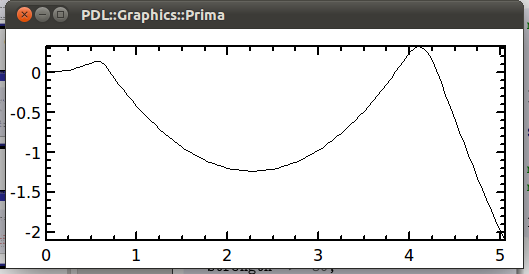
\includegraphics[width=0.8\linewidth]{example.png}
      }
    \end{column}
  \end{columns}
\end{frame}

\subsection{My Research: Ultrafast Electron Mircoscopy}

\begin{frame}{My Research: Ultrafast Electron Microscopy}
  \pgfdeclarelayer{background}
\pgfdeclarelayer{beam}
\pgfsetlayers{background,beam,main}

\begin{figure}
  \centering
  \begin{tikzpicture}
    [every pin edge/.style={white,thick}]
    \begin{pgfonlayer}{background}
      \node {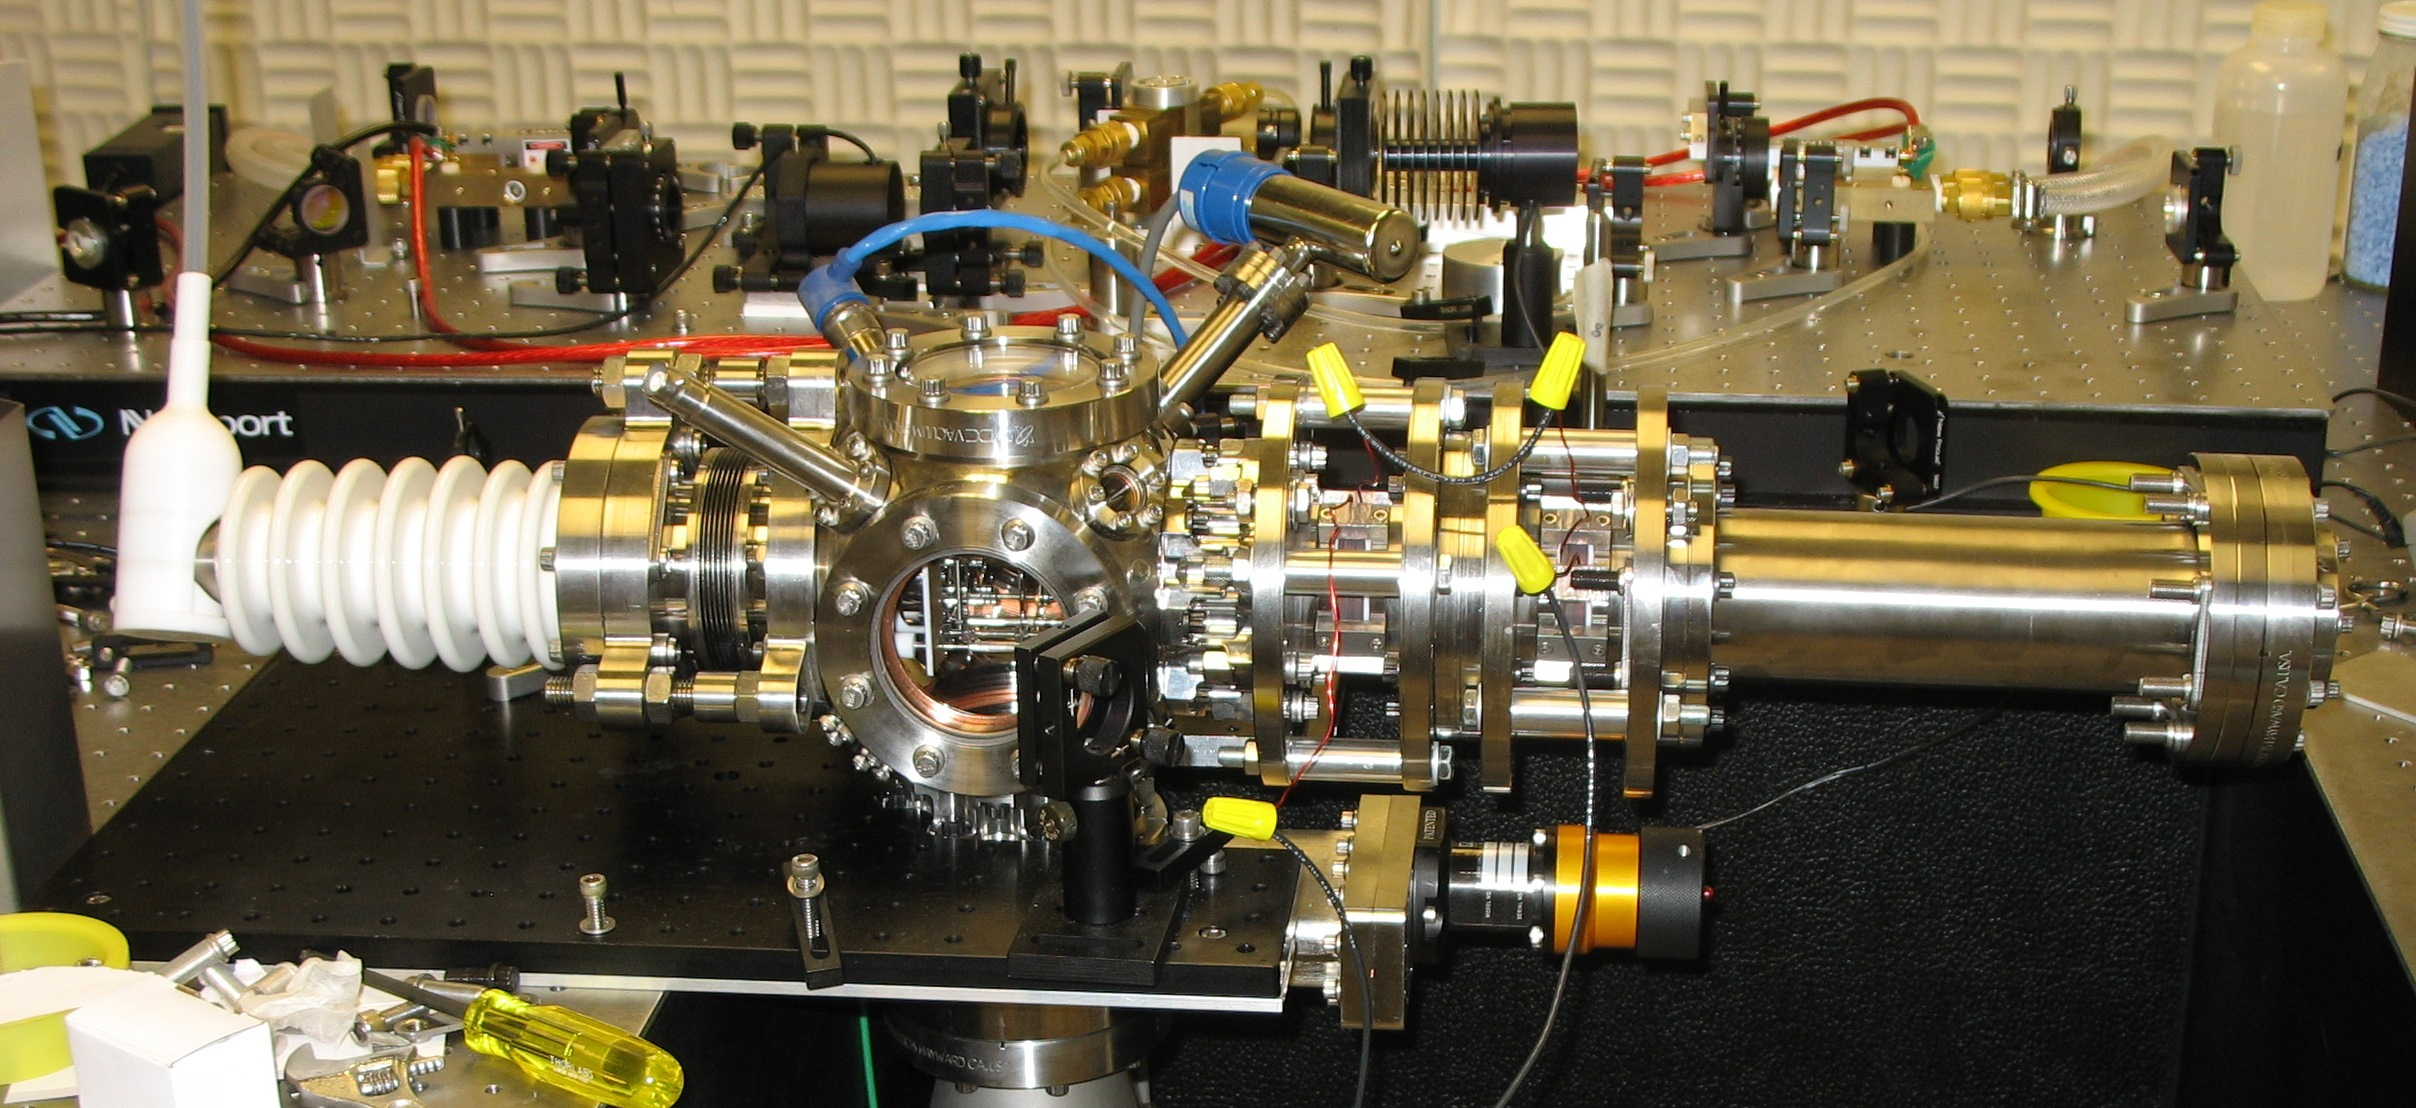
\includegraphics[width=0.9\linewidth]{column_lenses}};
    \end{pgfonlayer}
    \draw<2->
      [fill=orange] 
      (-2,-0.5)
      -- ++(0.2,0)
        node [midway,pin={below,fill=white:Photocathode}] {}
      -- ++(0,1)
        node [midway,inner sep=0.1] (source) {}
      -- ++(-0.2,0)
      -- cycle
    ;
    \draw<2->
      [fill=red]
      ($(source) + (2.35,0) $) node [inner sep=2mm] (lens1) {}
      arc (180:160:2)
      arc (20:-20:2)
        node (label lens1) {}
      arc (200:180:2)
    ;
    \draw<2->
      [fill=red]
      ($(source) + (3.4,0) $) node [inner sep=2mm] (lens2) {}
      arc (180:160:2)
      arc (20:-20:2)
        node (label lens2) {}
      arc (200:180:2)
    ;
    \node<2-> at ($(lens1)!0.5!(lens2) + (0,-1.5)$) (lens label) [red,fill=white] {Magnetic Lenses};
    \foreach \x in {1,2}
      \draw<2-> [white,thick] (lens label) -- (label lens\x);
    \draw<2-> 
      [fill=green!40]
      ($(source) + (6.5,0)$) node [inner sep=0] (detector) {}
        ellipse (0.2 and 0.5) 
          node at ($(source) + (6.5,-0.5)$) [pin={below,fill=white:Detector}] {}
    ;
    \draw<3->
      [green,very thick]
      (-5.2,-0.7)
      -- (-0.7,-0.7)
        node [pos=0.2,below=2mm,fill=white] {Laser}
      -- (source.east)
    ;
    \draw<5-> [fill=gray!60]
      ($(lens1)!0.5!(lens2) + (-0.05,0.5)$)
      node [pin={above,fill=white:{RF Cavity}}] {}
      rectangle ++(0.3,-1)
    ;
    \begin{pgfonlayer}{beam}
      \fill<4->
        [blue!40]
        (source)
        -- (lens1.north)
        -- (lens2.north)
        -- (detector.east)
          node [midway,above=5mm,fill=white] {Electron Beam}
        -- (lens2.south)
        -- (lens1.south)
      ;
    \end{pgfonlayer}
  \end{tikzpicture}
\end{figure}

\end{frame}

\begin{frame}{The Challenge: A Flexible Interface to a Complex Model}
  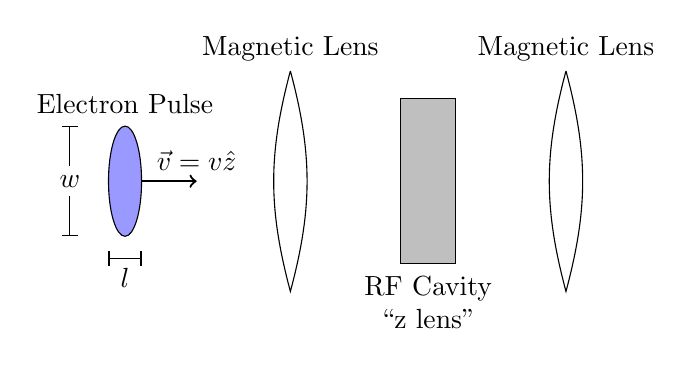
\begin{tikzpicture}[scale=0.7]
  \draw [fill=blue!40] (0,0) ellipse [x radius=3mm, y radius=1cm];
  \draw [|-|] (-1,1) -- ++(0,-2) node [pos=0.5,fill=white] {$w$};
  \draw [|-|] (-0.3,-1.4) -- ++(0.6,0) node [pos=0.5,below] {$l$};
  \node at (0, 1.4) {Electron Pulse};
  \draw [thick, ->] (0.3,0) -- ++ (1,0) node [above,pos=1] {$\vec{v} = v \hat{z}$};
  \draw 
    (3,2)
    to [out=-75,in=75] ++(0,-4)
    to [out=105,in=255] ++(0,4)
    node [above] {Magnetic Lens}
  ;
  \draw [fill=gray!50] (5,1.5) rectangle ++(1,-3);
  \node at (5.5,-2.2) [align=center] {RF Cavity\\``z lens''};
  \draw 
    (8,2)
    to [out=-75,in=75] ++(0,-4)
    to [out=105,in=255] ++(0,4)
    node [above] {Magnetic Lens}
  ;
\end{tikzpicture}

  \begin{itemize}
    \item<2-> Need: Compute dynamics of electron pulse ($w(t)$, $l(t)$)
    \item<3-> Note: Generation and optical elements add terms to DE
    \item<4-> Want: Representitive OO user-level interface
  \end{itemize}
\end{frame}

\begin{frame}{The ``State of the Art''}
  Old codes are
  \begin{itemize}
    \item lacking full 6D dynamics
    \item optimized for performance vs usablilty
    \item hard to customize
    \item near impossible to comprehend
  \end{itemize}
  \begin{block}<2->{\url{http://laacg.lanl.gov/laacg/services/download_sf.phtml}}
    \textbf{Getting Started with Poisson Superfish}\\
    \ldots We do not recommend trying to build an input file ``from scratch.'' Instead, find an example file that is similar to the problem you are trying to solve. Make a copy of the file and then make any necessary modifications to the geometry and options.
  \end{block}
\end{frame}

\begin{frame}{Other Attempts}
  \begin{columns}
    \begin{column}{0.49\linewidth}
      Mathematica:\\
      Pros:
      \uncover<2->{
      \begin{itemize}
        \item Can solve dynamics
        \item Pretty-printing of math for readability
      \end{itemize}
      }
      Cons:
      \uncover<3->{
      \begin{itemize}
        \item Closed-source and expensive!
        \item No OO and no key-value datatypes
        \item Still rather slow $\sim$2mins$/$sim
      \end{itemize}
      }
    \end{column}
    \begin{column}{0.49\linewidth}
      Modelica:\\
      Pros:
      \uncover<4->{
      \begin{itemize}
        \item Open-source, but behind close-source variants
        \item Unique OO language for physical simulation
        \item Classes have DEs as properties
      \end{itemize}
      }
      Cons:
      \uncover<5->{
      \begin{itemize}
        \item Lacks ``has-a'' relationship
        \item Composing DEs not trivial
        \item User-facing object instantiation not trivial
        \item Some numerical problems (?)
      \end{itemize}
      }
    \end{column}
  \end{columns}
\end{frame}

\begin{frame}{Example of \texttt{Physics::UEMColumn}}
  Back to Electron Column Modeling
  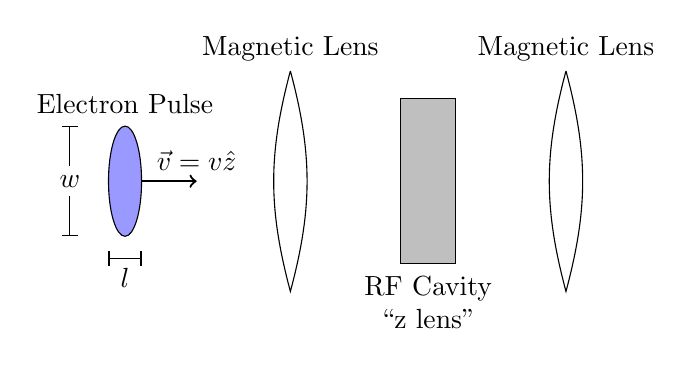
\begin{tikzpicture}[scale=0.7]
  \draw [fill=blue!40] (0,0) ellipse [x radius=3mm, y radius=1cm];
  \draw [|-|] (-1,1) -- ++(0,-2) node [pos=0.5,fill=white] {$w$};
  \draw [|-|] (-0.3,-1.4) -- ++(0.6,0) node [pos=0.5,below] {$l$};
  \node at (0, 1.4) {Electron Pulse};
  \draw [thick, ->] (0.3,0) -- ++ (1,0) node [above,pos=1] {$\vec{v} = v \hat{z}$};
  \draw 
    (3,2)
    to [out=-75,in=75] ++(0,-4)
    to [out=105,in=255] ++(0,4)
    node [above] {Magnetic Lens}
  ;
  \draw [fill=gray!50] (5,1.5) rectangle ++(1,-3);
  \node at (5.5,-2.2) [align=center] {RF Cavity\\``z lens''};
  \draw 
    (8,2)
    to [out=-75,in=75] ++(0,-4)
    to [out=105,in=255] ++(0,4)
    node [above] {Magnetic Lens}
  ;
\end{tikzpicture}

  \begin{itemize}
    \item As yet unreleased \code{Physics::UEMColumn}
    \begin{itemize}
      \item \url{https://github.com/jberger/Physics-UEMColumn}
    \end{itemize}
    \item Uses: \code{PerlGSL::DiffEq} on CPAN
    \begin{itemize}
      \item C-level solver of Perl-level DE closures
    \end{itemize}
  \end{itemize}
\end{frame}

\end{document}
